\chapter{Sensors}

A sensor is a device whose purpose is to detect events or changes in the environment and send the information to a computer processor. The processor will then use the sensor observations to perform more complex tasks.\\
In our case, we are using position and movement sensors in order to be able to localize the robot and keep track of its movements with respect to its starting position.\\

Nowadays MEMS\footnote{MEMS stands for "MicroElectroMechanical System"} sensors are widespread. MEMS is a technology which allows to miniaturize mechanical and electro-mechanical elements; therefore it enables to create very small sensors which can be integrated in circuits.\\

\section{Rotary Encoders}

A rotary encoder is a position sensor used for determining the angular position of a rotating shaft, it converts the angular position or motion of the shaft to analog or digital output signals.\\
There are two main types of rotary encoders, differing in the output signal: absolute and incremental.
\begin{itemize}
	\item Absolute encoders give in output a signal indicating the current shaft position;
	\item while incremental encoders provide information about the motion of the shaft, which is then processed to calculate the current shaft position.\\
\end{itemize}
In the following we will focus on incremental encoders as such are the ones used in the robot in consideration.\\

%https://www.mems-exchange.org/MEMS/what-is.html
%https://courses.cs.washington.edu/courses/cse466/14au/pdfs/lectures/MEMS%20Sensors.pdf

\begin{figure}[!ht]
	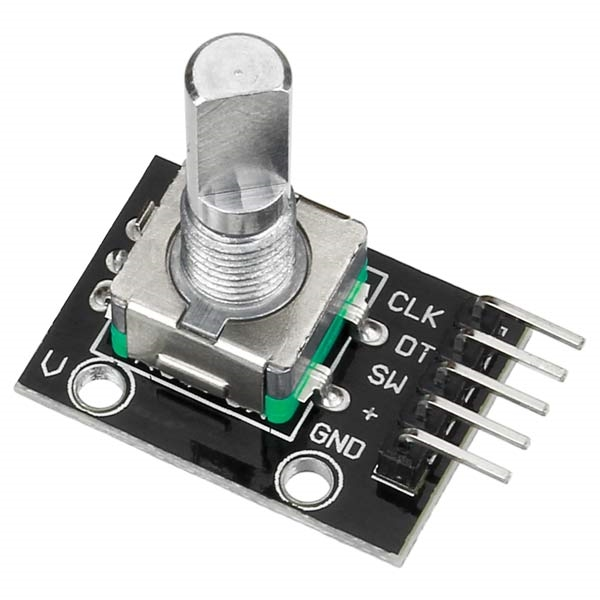
\includegraphics[scale=0.33]{enc_00}
	\captionsetup{justification=centering, margin=1.5cm}
	\centering
	\caption{Incremental Rotary Encoder}
	\centering
\end{figure}

\subsection{Incremental Rotary Encoders}\label{encoders_how_they_work}

As previously mentioned, an incremental encoder measure changes in position, but it does not keep track of absolute position.\\
It is also known as Quadrature Encoder since its A and B output signals are two square waves in quadrature.

%\begin{figure}[!ht]
%	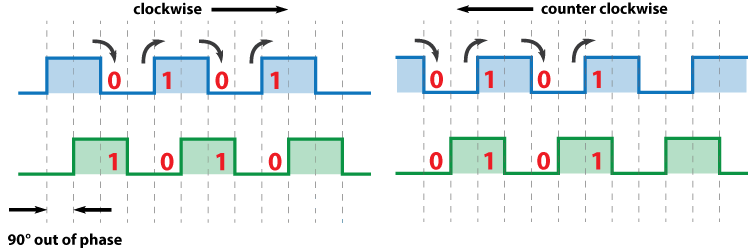
\includegraphics[scale=0.5]{enc_02}
%	\captionsetup{justification=centering, margin=1.5cm}
%	\centering
%	\caption{Incremental Encoder, output signals A and B.}
%	\centering
%\end{figure}

\begin{figure}[!ht]
	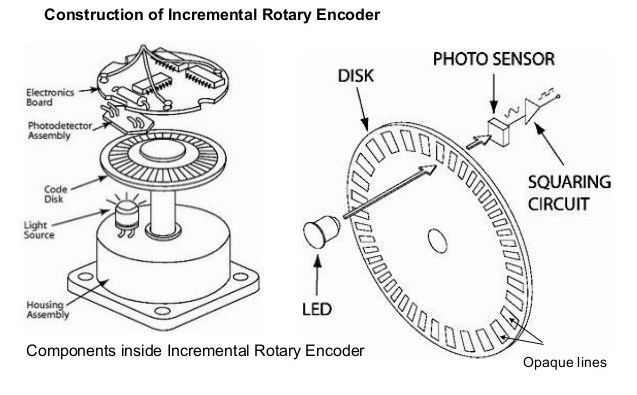
\includegraphics[scale=0.6]{enc_structure_00}
	\captionsetup{justification=centering, margin=1.5cm}
	\centering
	\caption{Encoder internal structure.}
	\centering
\end{figure}

%We can imagine the encoder as composed of a disk with evenly spaced contact zones, connected to a common pin and two other separate contact pins A and B. The disk rotates together with the shaft; while it rotates the pins A and B will start making contact with the common pin and the two square wave output signals will be generated accordingly.\\
The encoder is composed of a disk with evenly spaced opaque lines. On one side of the disk there is a light source, while on the other side there are two photodetectors, which are generating the signals A and B. The disk rotates together with the shaft, while it rotates the opaque lines will pass between the light source and the photodetectors generating the square waves.



\begin{figure}[htb]
 \centering
	\begin{subfigure}{0.2\textwidth}
		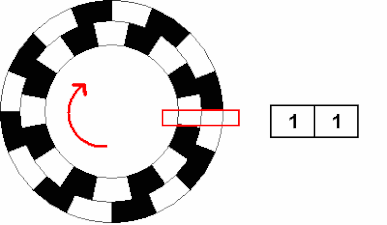
\includegraphics[width=\linewidth]{enc_principle_01}
	\end{subfigure}\hfil
	\begin{subfigure}{0.2\textwidth}
		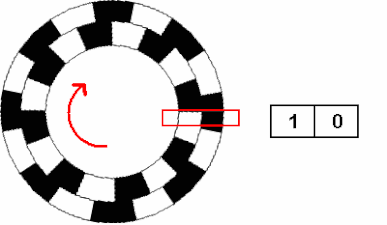
\includegraphics[width=\linewidth]{enc_principle_02}
	\end{subfigure}\hfil
	\begin{subfigure}{0.2\textwidth}
		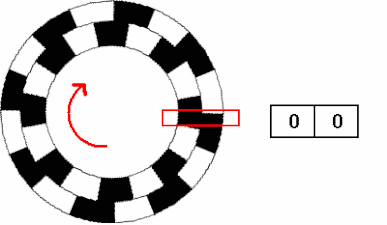
\includegraphics[width=\linewidth]{enc_principle_03}
	\end{subfigure}\hfil
	\begin{subfigure}{0.2\textwidth}
		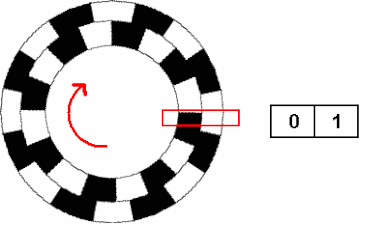
\includegraphics[width=\linewidth]{enc_principle_04}
	\end{subfigure}
	\captionsetup{justification=centering, margin=1.5cm}
	\caption{Generation of the square wave otuput pulses for clockwise rotations.}
\end{figure}

\begin{figure}[htb]
 \centering
	\begin{subfigure}{0.2\textwidth}
		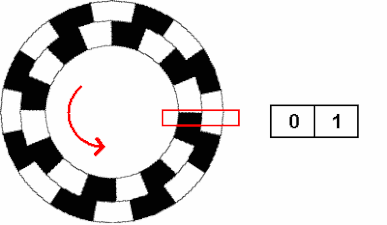
\includegraphics[width=\linewidth]{enc_principle_05}
	\end{subfigure}\hfil
	\begin{subfigure}{0.2\textwidth}
		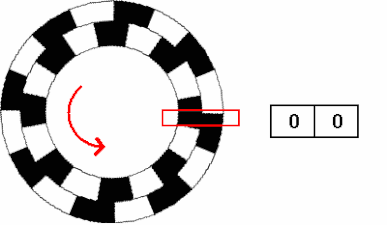
\includegraphics[width=\linewidth]{enc_principle_06}
	\end{subfigure}\hfil
	\begin{subfigure}{0.2\textwidth}
		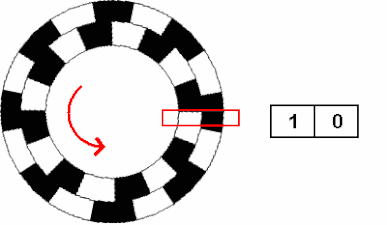
\includegraphics[width=\linewidth]{enc_principle_07}
	\end{subfigure}\hfil
	\begin{subfigure}{0.2\textwidth}
		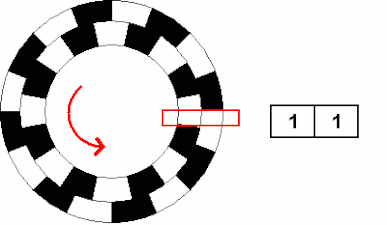
\includegraphics[width=\linewidth]{enc_principle_08}
	\end{subfigure}
	\captionsetup{justification=centering, margin=1.5cm}
	\caption{Generation of the square wave otuput pulses for anti-clockwise rotations.}
\end{figure}

The frequency of the pulses in the A and B output is directly proportional to the shaft rotational velocity; higher frequencies indicate rapid movement, whereas lower frequencies indicate slower speeds. Static, unchanging signals A and B indicate the encoder is motionless.


%https://www.youtube.com/watch?v=v4BbSzJ-hz4
%https://en.wikipedia.org/wiki/Incremental_encoder

\section{Inertial Measurement Unit}

There are mainly two categories of IMUs: stable platform systems and strapdown systems. The main difference between the two is the frame of reference in which the sensor operates.
\begin{itemize}
	\item In stable platform systems the inertial sensors are mounted on a platform isolated from any external motion; therefore the sensor always keep its alignment with the global frame.
	\item Strapdown systems instead are mounted rigidly on the platform, therefore the sensor is always aligned with the body frame (i.e. the navigation system's frame of reference).
\end{itemize}
In the following, we will consider strapdown systems as such is the one used in the robot we are considering.\\
Since the output is relative to the body frame, to keep track of the orientation gyroscope measurements must be integrated, and to keep track of the position accelerometer measurements are projected onto the global axis (using the orientation determined through the gyroscope) and then they are integrated\label{imu_integration}.\supercite{intro_inertial_navigation}
\begin{figure}[!ht]
	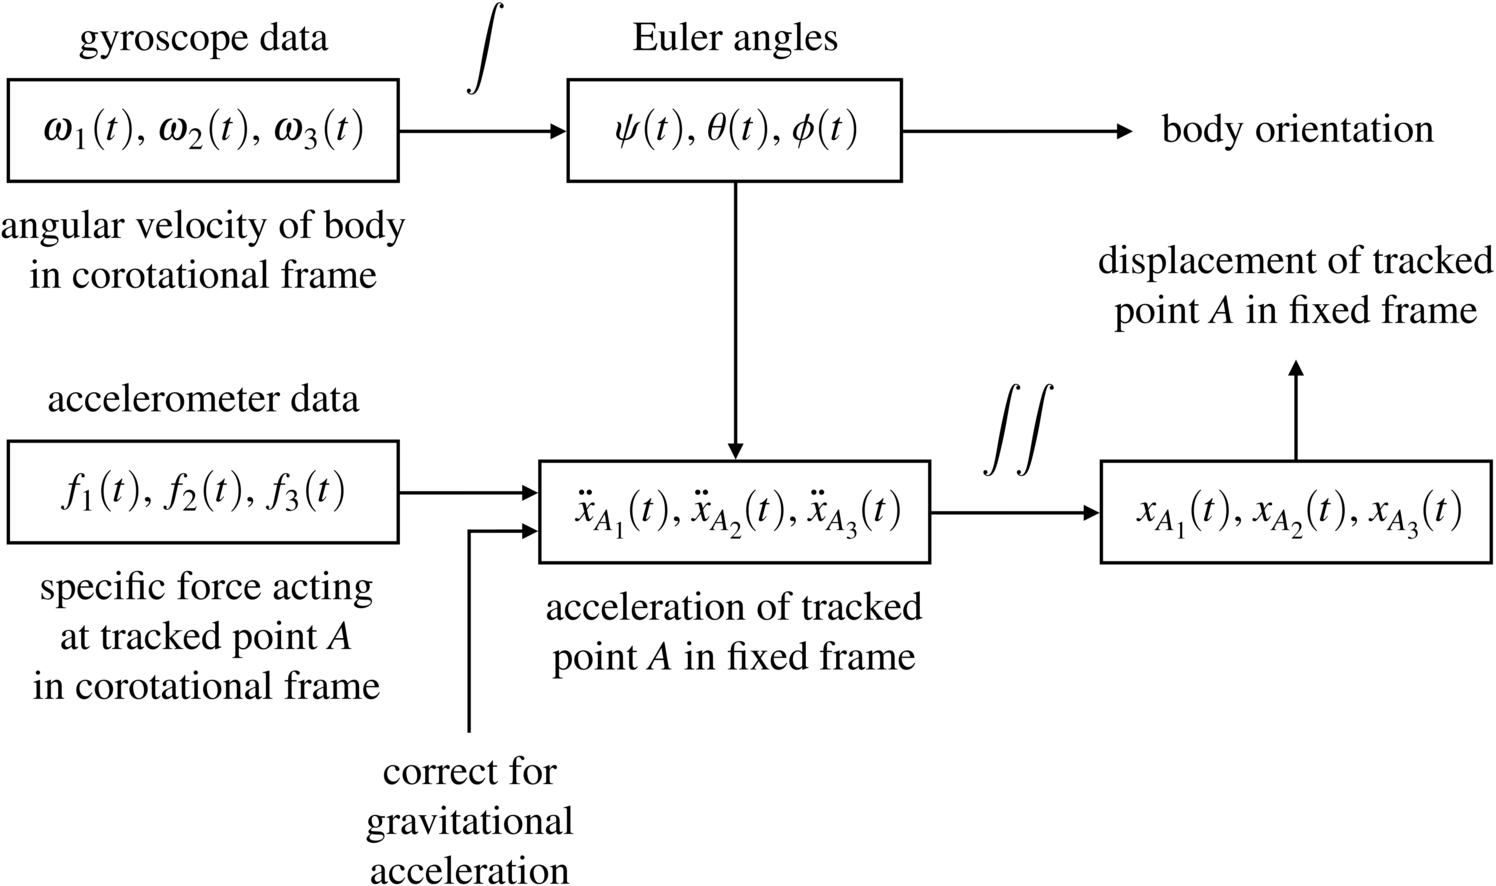
\includegraphics{imu_integration_40}
	\captionsetup{justification=centering, margin=1.5cm}
	\centering
	\caption{Strapdown Inertial Navigation Algorithm.}
	\centering
\end{figure}



\subsection{Gyroscope}

Gyroscopes are devices that measure rotational motion. While conventional gyroscopes measure orientation, most modern gyroscopes are rate-gyros measuring angular velocity.\\
\subsubsection{Mechanical Gyroscope}

A mechanical gyroscope consists of a spinning wheel mounted on two gimbals which allow it to rotate in all three axis. As an effect of the conservation of angular momentum, the spinning wheel will resist orientation changes. Hence when a gyroscope is subject to rotation, the wheel will keep rotating around the same rotational axis, while the angles between adjacent gimbals will change. Therefore to measure the orientation we have to measure angles between adjacent gimbals.\\
\begin{figure}[!ht]
	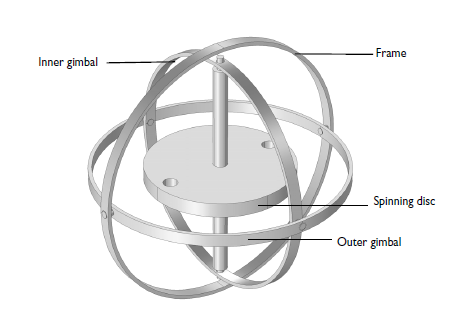
\includegraphics[scale=0.89]{mechanical_gyroscope}
	\captionsetup{justification=centering, margin=1.5cm}
	\centering
	\caption{Mechanical Gyroscope.}
	\centering
\end{figure}

\subsubsection{MEMS Gyroscope}

Unlike mechanical gyroscopes, MEMS gyros use the Coriolis effect to measure angular velocities. When a mass \textit{m} is moving with velocity \textit{v}, within a reference frame rotating at angular velocity \textit{$\omega$}, it experiences an apparent force:
\begin{gather*}
	F_c = -2m(\omega*v)
\end{gather*}

In MEMS gyros, vibrating elements are used to measure the Coriolis effect. In a simple configuration, there is a single mass allowed to vibrate along a drive axis; when the gyro is rotated, a second vibration occurs along the perpendicular sense axis due to the Coriolis effect. The angular velocity can be calculated from this second movement.

%\begin{figure}[!ht]
%	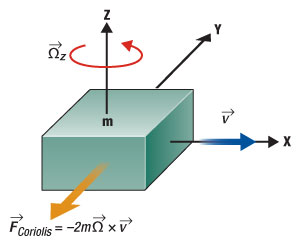
\includegraphics[scale=0.8]{mems_gyro_01}
%	\captionsetup{justification=centering, margin=1.5cm}
%	\centering
%	\caption{The Coriolis Force.}
%	\centering
%\end{figure}

\begin{figure}[htb]
 \centering
	\begin{subfigure}{0.45\textwidth}
		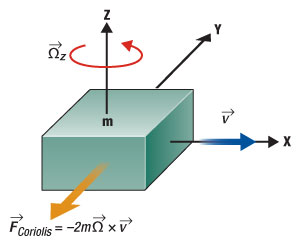
\includegraphics[width=\linewidth]{mems_gyro_01}
		\caption{The Coriolis Force.}
	\end{subfigure}\hfil
	\begin{subfigure}{0.45\textwidth}
		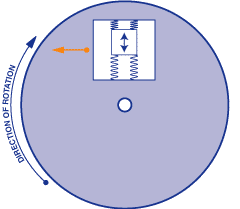
\includegraphics[width=\linewidth]{mems_gyro_02}
		\caption{MEMS Gyroscope.}
	\end{subfigure}
\end{figure}

Compared to conventional mechanical gyros, MEMS gyros are smaller and becoming cheaper, but they are not always as accurate as the former ones.

%\begin{figure}[!ht]
%	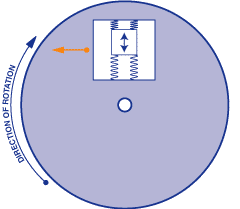
\includegraphics[scale=0.7]{mems_gyro_02}
%	\captionsetup{justification=centering, margin=1.5cm}
%	\centering
%	\caption{MEMS gyroscope.}
%	\centering
%\end{figure}

%references
%https://electroiq.com/2010/11/introduction-to-mems-gyroscopes/
%https://learn.sparkfun.com/tutorials/gyroscope [only image]
%supercite{intro_inertial_navigation}


\subsection{Accelerometer}

Accelerometers are devices that measure accelerations (i.e. the rate of change of the velocity of an object).

\subsubsection{Mechanical Accelerometer}

A mechanical accelerometer consists of a mass suspended by springs. When an acceleration occurs, as an effect of the principle of inertia, the mass will resist to any change in its velocity and the spring stretches with a force proportional to the acceleration (according to Newton's second law \textit{F = ma}). Therefore the distance the spring stretches can be used to measure the acceleration.

\begin{figure}[!ht]
	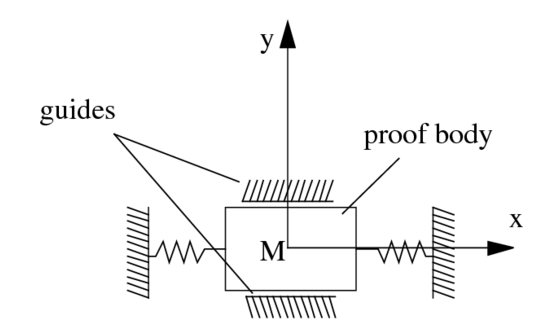
\includegraphics[scale=0.7]{mechanical_accelerometer_02}
	\captionsetup{justification=centering, margin=1.5cm}
	\centering
	\caption{Mechanical Accelerometer.}
	\centering
\end{figure}

\subsubsection{MEMS Accelerometer}

MEMS accelerometers usually contain capacitive plates internally. Some of these are fixed, while others are attached to springs and therefore able to move when subject to acceleration forces. As these plates move in relation to each other, the capacitance between them changes. Therefore measuring the capacitance we can determine the acceleration acting on the sensor.

%\begin{figure}[!ht]
%	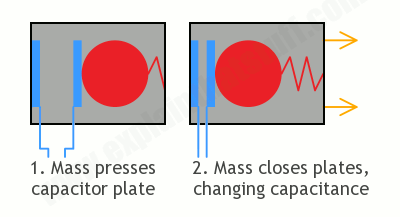
\includegraphics[scale=0.7]{capacitive_accelerometer}
%	\captionsetup{justification=centering, margin=1.5cm}
%	\centering
%	\caption{Capacitive Accelerometer.}
%	\centering
%\end{figure}

%\begin{figure}[!ht]
%	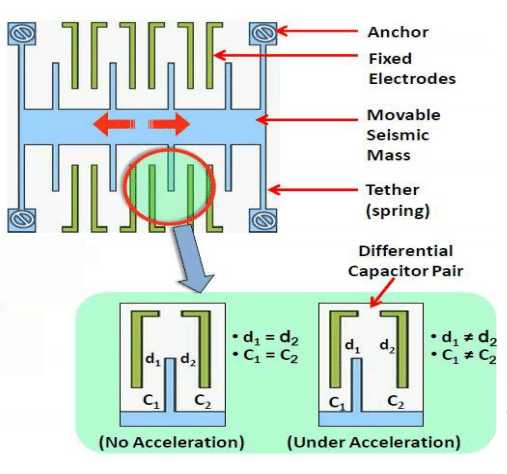
\includegraphics[scale=0.7]{mems_accelerometer_00}
%	\captionsetup{justification=centering, margin=1.5cm}
%	\centering
%	\caption{Capacitive Accelerometer.}
%	\centering
%\end{figure}

\begin{figure}[htb]
 \centering
	\begin{subfigure}{0.48\textwidth}
		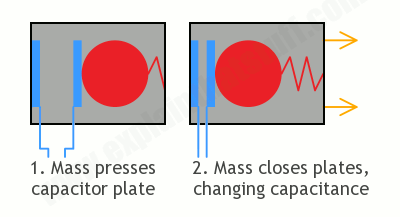
\includegraphics[width=\linewidth]{capacitive_accelerometer}
		\caption{Capacitive Accelerometer.}
	\end{subfigure}\hfil
	\begin{subfigure}{0.48\textwidth}
		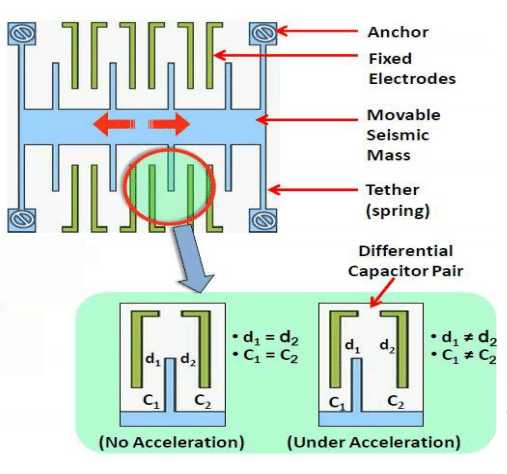
\includegraphics[width=\linewidth]{mems_accelerometer_00}
		\caption{MEMS Accelerometer.}
	\end{subfigure}
\end{figure}

%references
%https://www.explainthatstuff.com/accelerometers.html [mechanical]
%http://mafija.fmf.uni-lj.si/seminar/files/2007_2008/MEMS_accelerometers-koncna.pdf[mems]
%https://www.youtube.com/watch?v=KZVgKu6v808[mems]

\subsection{MEMS Sensors Error Characteristics}\label{mems_errors}

MEMS sensors are subject to many possible different errors; in the following we will explain only the ones we took in consideration calibrating our sensors (we will describe the calibration process we used in Section \ref{imu_calib}).
\begin{itemize}
	\item \textbf{Constant Biases}. The bias of a MEMS sensor is the average value it outputs in a motionless state.
	\item \textbf{Scale Factor Erros}. The scale factor should convert the digital quantity measured by each sensor into real physical quantities (e.g, accelerations and gyro rates). Unfortunately, MEMS based IMUs are affected by non-accurate scaling; therefore the scale factor tends to be slightly different from the one expected, and the 3-axes of the same sensor may have different scale factors.
	\item \textbf{Thermo-Mechanical White Noise}. The output of MEMS sensors is also affected by a zero-mean thermo-mechanical noise.
\end{itemize}
